\documentclass[a4paper,12pt]{article}
\usepackage{amsmath, amssymb}
\usepackage{siunitx}
\usepackage{hyperref}
\usepackage{graphicx}
\usepackage{float}
\usepackage[a4paper, top=0.5in, bottom=0.5in, left=1in, right=1in]{geometry}
\usepackage{xcolor}
\usepackage{colortbl}
\usepackage{titlesec}
\usepackage{fontspec}
\usepackage{tikz}
\usepackage{lipsum} % For dummy text, remove this for your actual report
\usepackage{listings}
\usepackage{subcaption}
\usepackage{tcolorbox}
\usepackage{fancyhdr}
\lstset{
    language=Python,        % Specify the language
    basicstyle=\ttfamily,   % Basic font style
    keywordstyle=\color{blue}\bfseries, % Keywords style
    commentstyle=\color{green},         % Comments style
    stringstyle=\color{red},            % Strings style
    numbers=left,                      % Add line numbers
    numberstyle=\tiny,                 % Line number style
    stepnumber=1,                      % Step between line numbers
    frame=single,                      % Add a frame around the code
    breaklines=true                    % Allow breaking long lines
}

\definecolor{myblue}{rgb}{0.1, 0.2, 0.7}
\definecolor{mygreen}{rgb}{0.1, 0.6, 0.1}
\definecolor{myred}{rgb}{0.7, 0.2, 0.2}
\definecolor{lightblue}{rgb}{0.8, 0.9, 1}
\definecolor{mygold}{rgb}{0.8, 0.6, 0.1}
\definecolor{mygray}{rgb}{0.9, 0.9, 0.9}

% Customize title formatting
\titleformat{\title}[block]
  {\normalfont\Huge\bfseries\color{myblue}}{}{0em}{}

\titleformat{\author}[block]
  {\normalfont\LARGE\itshape\color{mygreen}}{}{0em}{}

% Custom header line
\newcommand{\myheader}{
    \noindent\rule{\textwidth}{1pt}\\[0.4cm]
}

% Title page design
\begin{document}

% Title Page
\begin{titlepage}
    \centering
    
    \vspace*{2cm}
    
    % Title
    {\Huge \bfseries \textcolor{myblue}{Lab Report : Transient Response of LC circuits}}\\[0.5cm]
    {\LARGE \textit{\textcolor{red}{Analysing the LC circuit response}}\\[1.5cm]
    
    % Author names
    \noindent
    \textbf{\Huge Krishna Patil-EE24BTECH11036}\\[0.3cm]
    \textbf{\Huge Deepak Ahirwar-EE24BTECH11014}\\[1.5cm]
    
    % Institution name
    {\LARGE \textit{Electrical Department, IIT-Hyderabad}}\\[2cm]
    
    \vfill
    
    % Date
    {\LARGE \today}
    
    % Footer - with gradient line and custom footer text
    \vfill
    \myheader
    \centering
    \textcolor{mygold}{\Large \textit{Experiment conducted as part of ELectric Circuits Lab Coursework.}}
    
\end{titlepage}

\pagestyle{fancy}
\fancyhf{}
\rhead{\textcolor{purple}{LC Circuit Analysis}}
\lhead{\textcolor{orange}{Electric Circuits Lab}}
\cfoot{\textcolor{red}{\thepage}}

\begin{tcolorbox}[colframe=red!70!black,colback=yellow!10!white,title=\textbf{\textcolor{red}{Objective}}]
The objective of this experiment is to investigate the transient response of an LC circuit, analyze its oscillatory behavior, determine the natural frequency ($\Omega_n$), and evaluate the damping ratio ($\xi$) using both theoretical and experimental methods.
\end{tcolorbox}

\begin{tcolorbox}[colframe=blue!70!black,colback=cyan!10!white,title=\textbf{\textcolor{blue}{Equipment Required}}]
\begin{itemize}
    \item \textcolor{green}{100 $\mu$F capacitor}  
    \item \textcolor{green}{Largest available inductor (denoted as L)}  
    \item \textcolor{green}{Small resistor (for optional damping analysis)}  
    \item \textcolor{green}{DC power supply}  
    \item \textcolor{green}{Digital oscilloscope}  
    \item \textcolor{green}{Function generator}  
    \item \textcolor{green}{Connecting wires and probes}  
    \item \textcolor{green}{Multimeter for component verification}  
\end{itemize}
\end{tcolorbox}

\section{\textcolor{red}{Theory}}
\begin{tcolorbox}[colframe=purple!70!black,colback=magenta!10!white]
An LC circuit consists of an inductor (L) and a capacitor (C) connected in parallel or series. The system follows a second-order differential equation:
\begin{equation}
    \frac{d^2V}{dt^2} + \frac{R}{L} \frac{dV}{dt} + \frac{1}{LC} V = 0
\end{equation}
\end{tcolorbox}

\section{\textcolor{red}{Procedure}}
\begin{tcolorbox}[colfame=orange!70!black,colback=yellow!20!white]
\begin{enumerate}
    \item \textbf{Precharge the Capacitor:}
    \begin{itemize}
        \item Connect the 100 $\mu$F capacitor to a 5V DC power supply.
        \item Verify the capacitor’s voltage using a multimeter before proceeding.
    \end{itemize}
    \item \textbf{Construct the LC Circuit:}
    \begin{itemize}
        \item Select the largest available inductor.
        \item Connect the capacitor in parallel with the inductor.
    \end{itemize}
    \item \textbf{Capture the Transient Response:}
    \begin{itemize}
        \item Attach the oscilloscope probes across the capacitor terminals.
        \item Observe and record the oscillations.
    \end{itemize}
\end{enumerate}
\end{tcolorbox}

\section{\textcolor{red}{Observations and Analysis}}
\begin{tcolorbox}[colframe=teal!70!black,colback=cyan!10!white]
\begin{itemize}
    \item \textcolor{blue}{Captured transient response waveform from the oscilloscope.}
    \item \textcolor{blue}{Measured oscillation period and compared it with theoretical expectations.}
\end{itemize}
\end{tcolorbox}

\section{\textcolor{red}{Images of Responses}}
\begin{tcolorbox}[colframe=black!70!black,colback=gray!10!white,title=\textbf{\textcolor{white}{Oscilloscope Waveforms and Circuit Images}}]
\begin{center}
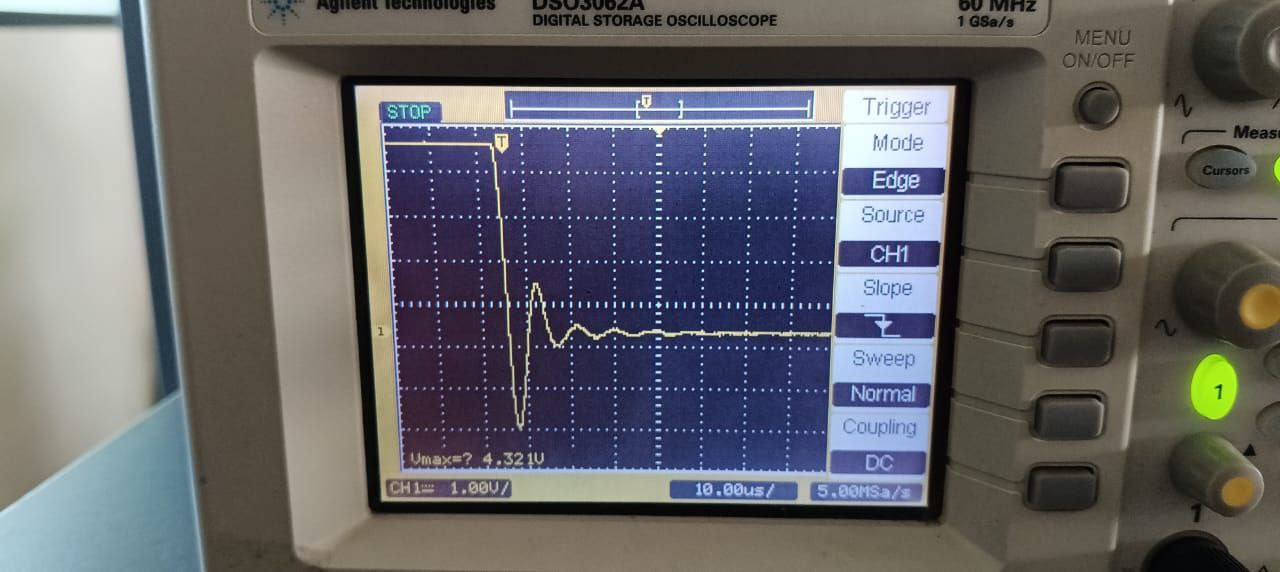
\includegraphics[width=0.8\textwidth]{response_image1.png} \
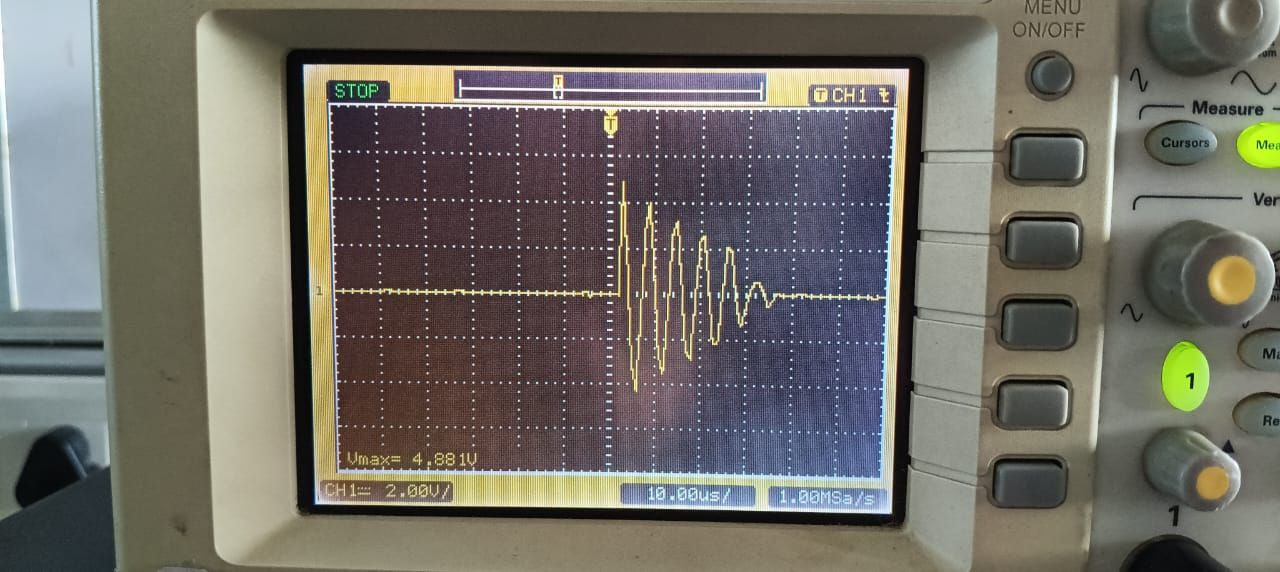
\includegraphics[width=0.8\textwidth]{response_image2.png}
\end{center}
\textcolor{black}{Above images depict the transient response captured during the experiment.}
\end{tcolorbox}

\section{\textcolor{red}{Conclusion}}
\begin{tcolorbox}[colframe=red!70!black,colback=yellow!10!white]
The experimentally observed natural frequency closely matched theoretical values. The presence of resistance introduced measurable damping effects.
\end{tcolorbox}

\section{\textcolor{red}{Safety Precautions}}
\begin{tcolorbox}[colframe=purple!70!black,colback=magenta!10!white]
\begin{itemize}
    \item Handle charged capacitors carefully to avoid accidental discharges.
    \item Ground the oscilloscope properly for accurate and safe measurements.
\end{itemize}
\end{tcolorbox}

\section{\textcolor{red}{References}}
\begin{tcolorbox}[colframe=green!70!black,colback=yellow!10!white]
\begin{itemize}
    \item \textit{Transient Response of an LC Circuit}.
    \item Circuit analysis textbooks and academic literature.
\end{itemize}
\end{tcolorbox}

\end{document}

r
